\chapter{Specialising and optimising xDSL pattern rewriting}
\label{chap:specialising-optimising-pattern-rewriting}

%% Introduction and goals (make faster and only constrained by language runtime)
% Hook
In \autoref{chap:measuring-compiler-performance}, we constructed a set of experiments to empirically compare the current performance of the xDSL and \ac{mlir} compiler frameworks.
% Argument
Our overall aim is to use these experiments to contrast the performance of static and dynamic languages for the implementation of user-extensible compiler frameworks, using \ac{mlir} and xDSL as proxies for these two categories respectively.
However, the experiments so far measure a combination of the effects of dynamism in the language runtime and implementation details of the framework, with the former obscuring our goal of measuring the latter.
% Link
In order to use the frameworks for our aims, our measurements must be as independent of implementation details as possible.

% Hook
In this chapter, we meet this requirement by specialising the xDSL framework to implement only a single workload.
% Argument
In this process, we manually identify and remove computation performed by the framework which is unnecessary to its execution of this workload. This computation broadly falls into two categories. The first is functionality which. % TODO: Fill in
The second is calculating and checking values which are known as runtime invariants for the selected workload. % TODO: Fill in
By eliminating both of these performance overheads, we reach an implementation representative of the best-case performance of Python for this workload.
% Link
The benefits of this specialisation are twofold. Firstly it reveals inefficiencies in xDSL which can be optimised to improve the general performance of the framework. Secondly, it provides a true performance baseline for dynamic languages irrespective of implementation details which can be used to quantify the impact of dynamism in \autoref{chap:dynamism-pattern-rewriting}.


\section{Micro-benchmarks}
\label{sec:specialising-ubenchmarks}

%% Link back to micro-benchmarks and summarise section
% Hook
An important component of our experimental suite is micro-benchmarks, measuring the performance of procedures fundamental to xDSL and \ac{mlir}.
% Argument
The small size of these micro-benchmarked procedures makes them tractable first targets for manual specialisation and optimisation, with the performance impact of this process easily characterised by repeating the micro-benchmark.
By manually examining the traces of their execution, we can identify and eliminate any unnecessary computation in the current implementation.
% Link
Having done this, we re-run the micro-benchmarks to quantify the performance of the specialised implementation, facilitating comparison of the language runtime only for user-extensible compiler framework workloads.
% In this section, we examine the specialisation process for these micro-benchmarks in detail. % TODO: Add more stuff here!!


\subsection{Operation instantiation}
\label{sec:specialising-ubenchmarks-instantiation}

%% Re-introduce microbenchmark
% Hook
The first micro-benchmark discussed was instantiating operations, one of the central data structures in both xDSL and \ac{mlir}.
% Argument
The idiomatic way to do this in xDSL is directly instantiating a new Python object.
This invokes the \mintinline{python3}{__new__} method to construct an empty class, then the \mintinline{python3}{__init__} method to initialise it, and optionally \mintinline{python3}{__post_init__} following initialisation.
In xDSL, this instantiation process includes a large amount of logic (\autoref{fig:ubenchmark-hastrait-xdsl-viztracer}), including verifying attributes and building properties of the operation.
However, in many instances this verification is unneeded as it is already known as a runtime invariant, and the building process can similarly be simplified as the structure can be inferred.
% Link
As such, specialisation to remove this overhead can vastly reduce the complexity and hence improve performance (\autoref{fig:ubenchmark-gettrait-xdsl-viztracer}).

\begin{figure}[H]
    \centering
    \begin{subfigure}[b]{\textwidth}
        \centering
        \begin{tikzpicture}
            \node[anchor=south west,inner sep=0] (image) at (0,0) {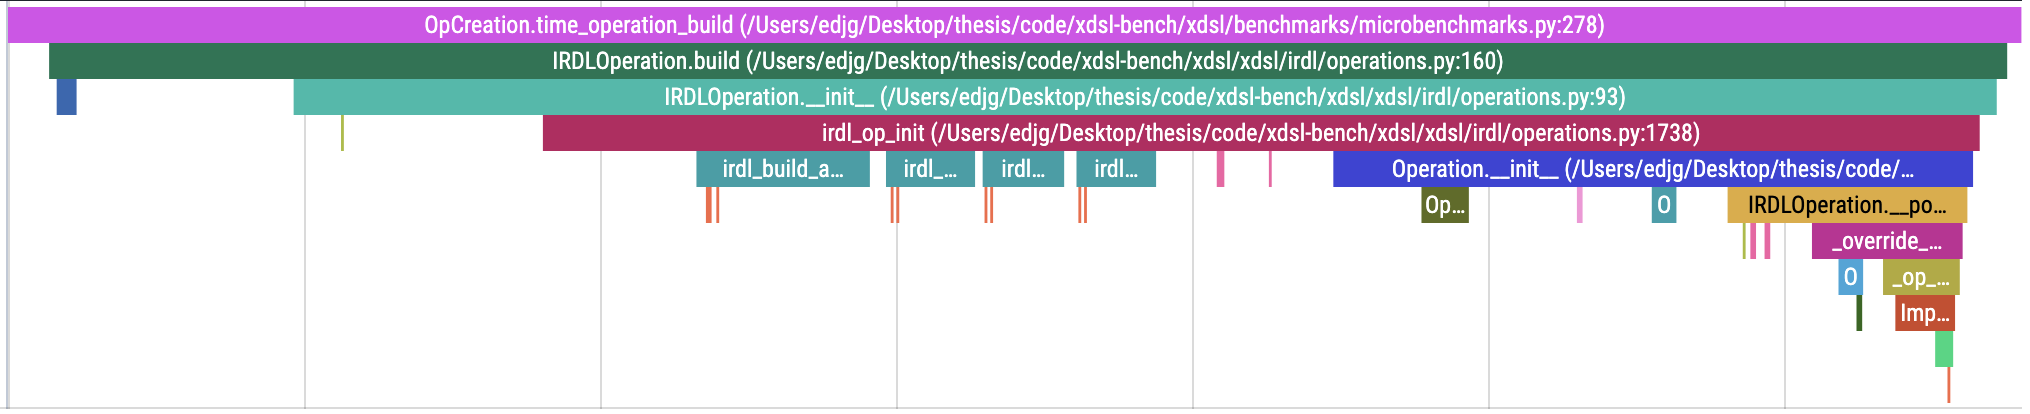
\includegraphics[width=\textwidth]{images/specialising_optimising_xdsl_rewriting/original_empty_create}};
            \node[circledstyle, fill=pairedOneLightBlue] at (6.25,1.25) {A};
            \node[circledstyle, fill=pairedTwoDarkBlue] at (14,0.75) {B};
        \end{tikzpicture}
        % \begin{tikzpicture}[remember picture,overlay]
        %     % \node[circledstyle,draw] at ([xshift=2cm,yshift=1cm]current page.center) {A};
        %     \node[circledstyle, fill=pairedOneLightBlue] ([xshift=2cm,yshift=5cm]current page.center) {A};
        % \end{tikzpicture}
        \captionsetup{width=0.8\textwidth}
        \caption{The default constructor has a high overhead, calculating known invariants and .}
        \label{fig:ubenchmark-hastrait-xdsl-viztracer}
    \end{subfigure}
    \begin{subfigure}[b]{\textwidth}
        \centering
        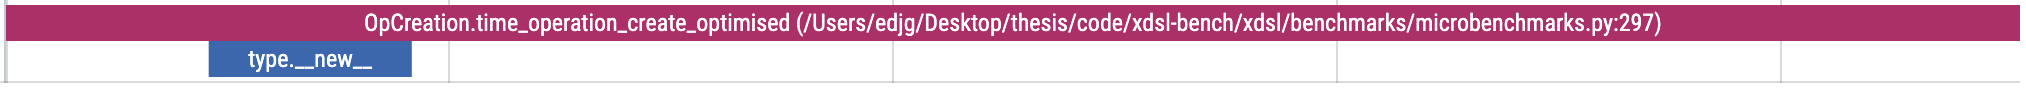
\includegraphics[width=\textwidth]{images/specialising_optimising_xdsl_rewriting/optimised_empty_create}
        \captionsetup{width=0.8\textwidth}
        \caption{The same object can be constructed with significantly less logic.}
        \label{fig:ubenchmark-gettrait-xdsl-viztracer}
    \end{subfigure}
    \caption{\texttt{viztracer} traces of xDSL instantiating an \texttt{EmptyOp} before (top) and after (bottom) specialisation.}
    \label{fig:ubenchmark-hasgettrait-xdsl-viztracer}
\end{figure}

%% Describe specialisation/optimisation
% Hook
Examining the above trace, we can visually identify components which take a large proportion of runtime, and may represent unnecessary computation.
% Argument
For example, the xDSL constructor for \mintinline{python3}{IRDLOperation}s invokes logic with significant overhead building and filtering properties of the operation \circledbase{pairedOneLightBlue}{A}. However, in this example of the empty operation, this logic does not change the constructed object. Because of this, eliding this logic results in a specialised version of the operation which generates the same output using less computation by applying domain knowledge.
In addition to this, \ac{mlir}'s core operations are not \ac{irdl} based, unlike xDSL, meaning this overhead is implementation specific.
Similarly, the post-constructor includes logic for context-managed builders \circledbase{pairedTwoDarkBlue}{B}, which is again unrelated to the empty operation case and not present in \ac{mlir}.
% Link
To avoid this overhead through specialisation, we move from the idiomatic constructor (Listing \ref{listing:ubenchmark-xdsl-constant-constructor}) to directly modifying xDSL's underlying data structures (Listing \ref{listing:ubenchmark-xdsl-constant-direct}).


\begin{figure}[H]
    \begin{subfigure}[b]{0.5\textwidth}
       \centering
        \begin{minted}[fontsize=\footnotesize]{text}
            EmptyOp()
        \end{minted}
        % ConstantOp(
        %         IntegerAttr(
        %             100,
        %             i32
        %         )
        %     )
        \footnotesize\vspace{3.5em}
        \caption{Instantiation with constructors.}
        \label{listing:ubenchmark-xdsl-constant-constructor}
    \end{subfigure}
    \hfill
    \begin{subfigure}[b]{0.5\textwidth}
        \centering
        \begin{minted}[breakanywhere,fontsize=\footnotesize]{text}
            empty_op = EmptyOp.__new__(EmptyOp)
            empty_op._operands = tuple()
            empty_op.results = tuple()
            empty_op.properties = {}
            empty_op.attributes = {}
            empty_op._successors = tuple()
            empty_op.regions = tuple()
        \end{minted}
            % int_attr = IntAttr.__new__(IntAttr)
            % object.__setattr__(int_attr, "data", 100)
            % integer_attr = IntegerAttr.__new__(IntegerAttr)
            % object.__setattr__(integer_attr, "parameters", (int_attr, i32))
            % constant_op = ConstantOp.__new__(ConstantOp)
            % constant_op._operands = tuple()
            % constant_op.results = (OpResult(i32, constant_op, 0),)
            % constant_op.properties = {"value": integer_attr}
            % constant_op.attributes = {}
            % constant_op._successors = []
            % constant_op.regions = tuple()
        \caption{Instantiation by direct manipulation of xDSL's data structures.}
        \label{listing:ubenchmark-xdsl-constant-direct}
    \end{subfigure}
    \captionsetup{name=Listing}
    \caption{Approaches to instantiating an empty operation.}
    \label{listing:ubenchmark-xdsl-constant}
\end{figure}

%% Specialised performance and lessons learnt
% Hook
Through this process of specialisation, we can improve the performance of this micro-benchmark by up to $26\times$ (\autoref{tab:ubenchmark-instantiation-optimised}).
% Argument
From this example, we can see that xDSL's design goal of a simple, expressive API is antagonistic with the performance of its implementation. By specialising the implementation to the workload, directly invoking only the required instructions, we can achieve significant performance improvements. We argue that this specialisation approaches the upper bound of performance for this workload as a result of the constraints of the language runtime.
% Link

\begin{table}[H]
  \caption{Specialisation improves xDSL's operation instantiation performance by $26\times$, lifting it from $83\times$ to $3\times$ slower than \ac{mlir}.}
  \label{tab:ubenchmark-instantiation-optimised}
  \centering
  \begin{tabular}{ccc}
    \toprule
    \textbf{MLIR [ns]} & \textbf{xDSL [ns]} & \textbf{Optimised xDSL [ns]} \\
    \midrule
    $153 \pm 0.5$ & $12700 \pm 1810$ & $477 \pm 385$ \\
    % $357 \pm 0.5$ & $33400 \pm 3680$ & $1830 \pm 774$ \\
    \bottomrule
  \end{tabular}
\end{table}


%% Compare performance and number of bytecode/assembly operations














\subsection{Operation trait checks}
\label{ssec:specialising-ubenchmarks-trait}

%% Re-introduce microbenchmark
% Hook
The second micro-benchmark discussed in \autoref{sec:ubenchmark} was checking traits on operations, and was measured to perform $\times$ worse in xDSL than \ac{mlir}.
% Argument
Similarly to the operation instantiation micro-benchmark, this slow-down results from a high proportion of method's logic not implementing the core functionality (\autoref{fig:ubenchmark-hastrait-original-viztracer}). In this case, this logic improves the expressivity of the API, supporting both concrete objects and types as arguments, along with handling the edge case of unregistered operations. However, this logic lies on the hot path of execution, and again these properties are known as runtime invariants. As such, specialisation can again be leveraged to remove this implementation overhead (\autoref{fig:ubenchmark-hastrait-optimised-viztracer}).
% Link

\begin{figure}[H]
    \centering
    \begin{subfigure}[b]{\textwidth}
        \centering
        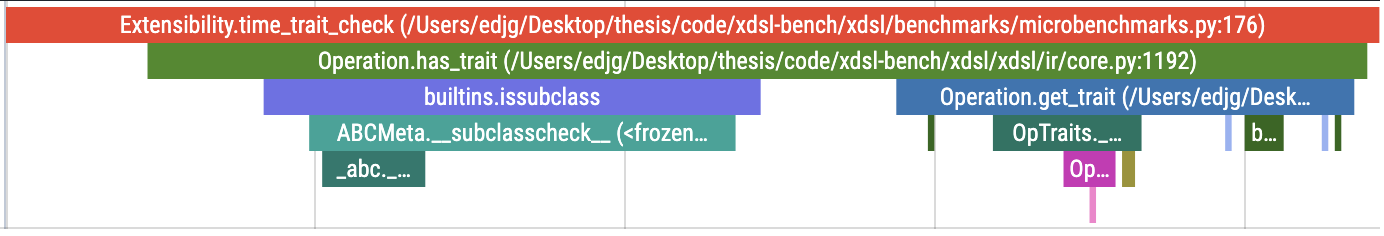
\includegraphics[width=\textwidth]{images/specialising_optimising_xdsl_rewriting/original_hastrait.png}
        \captionsetup{width=0.8\textwidth}
        \caption{\mintinline{python}{issubclass} and \mintinline{python}{isinstance} checks, type \mintinline{python}{cast}ing, and constructing iterators constitutes over three quarters of xDSL's \mintinline{python}{has_trait}s runtime.}
        \label{fig:ubenchmark-hastrait-original-viztracer}
    \end{subfigure}
    \begin{subfigure}[b]{\textwidth}
        \centering
        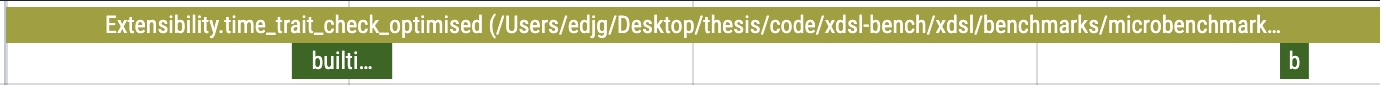
\includegraphics[width=\textwidth]{images/specialising_optimising_xdsl_rewriting/optimised_hastrait.png}
        \captionsetup{width=0.8\textwidth}
        \caption{Specialisation to narrow the interface and optimisation to avoid extraneous work on hot paths can significantly accelerate \mintinline{python}{has_trait}.}
        \label{fig:ubenchmark-hastrait-optimised-viztracer}
    \end{subfigure}
    \caption{\texttt{viztracer} traces of xDSL's \mintinline{python}{has_trait} method.}
    \label{fig:ubenchmark-hastrait-viztracer}
\end{figure}


%% Describe specialisation/optimisation
% Hook
% Argument
% Link

\begin{figure}[H]
    \begin{subfigure}[b]{0.45\textwidth}
       \centering
        \begin{minted}[fontsize=\footnotesize,escapeinside=$$]{text}
            @classmethod
            def has_trait(
                cls,
                trait: type[OpTrait] | OpTrait,
                *,
                value_if_unregistered: bool = True,
            ) -> bool:
                from xdsl.dialects.builtin import UnregisteredOp $\circledbase{pairedOneLightBlue}{1}$

                if issubclass(cls, UnregisteredOp):
                    return value_if_unregistered

                return cls.get_trait(trait) is not None $\circledbase{pairedTwoDarkBlue}{2}$
        \end{minted}
        \footnotesize\vspace{1.5em}
        \caption{Outer \mintinline{python}{has_trait} method.}
        \label{listing:ubenchmark-trait-checks-xdsl-has}
    \end{subfigure}
    \hfill
    \begin{subfigure}[b]{0.45\textwidth}
        \centering
        \begin{minted}[breakanywhere,fontsize=\footnotesize,escapeinside=$$]{text}
            @classmethod
            def get_trait(
                cls,
                trait: type[OpTraitInvT] | OpTraitInvT
            ) -> OpTraitInvT | None:
                if isinstance(trait, type): $\circledbase{pairedThreeLightGreen}{3}$
                    for t in cls.traits:
                        if isinstance(t, cast( $\circledbase{pairedFourDarkGreen}{4}$
                            type[OpTraitInvT], trait
                        )):
                            return t
                else:
                    for t in cls.traits:
                        if t == trait:
                            return cast(OpTraitInvT, t)
                return None
        \end{minted}
        \caption{Inner \mintinline{python}{get_trait} method.}
        \label{listing:ubenchmark-trait-checks-xdsl-get}
    \end{subfigure}
    \vspace{1em}
    \captionsetup{name=Listing}
    \caption{xDSL methods implementing trait check functionality.}
    \label{listing:ubenchmark-trait-checks-xdsl}
\end{figure}

\begin{figure}[H]
    \centering
    \begin{subfigure}[b]{0.45\textwidth}
       \centering
        \begin{minted}[fontsize=\footnotesize]{text}
            for t in OP.traits._traits:
                if isinstance(t, TRAIT):
                    return True
            return False
        \end{minted}
        \footnotesize\vspace{2em}
        \captionsetup{name=Listing}
        \caption{xDSL's modified \mintinline{python}{has_trait} method.}
        \label{listing:ubenchmark-trait-checks-both-xdsl}
    \end{subfigure}
    \hfill
    \begin{subfigure}[b]{0.45\textwidth}
        \centering
        \begin{minted}[breakanywhere,fontsize=\footnotesize]{text}
            TypeID traitIDs[] = {TypeID::get<Traits>()...};
            for (unsigned i = 0, e = sizeof...(Traits); i != e; ++i)
                if (traitIDs[i] == traitID)
                    return true;
            return false;
        \end{minted}
        \captionsetup{name=Listing}
        \caption{\ac{mlir}'s \mintinline{c++}{has_trait} method.}
        \label{listing:ubenchmark-trait-checks-both-mlir}
    \end{subfigure}
    \vspace{1em}
    \captionsetup{name=Listing}
    \caption{xDSL and \ac{mlir} methods searching trait arrays.}
    \label{listing:ubenchmark-trait-checks-both}
\end{figure}

%% Specialised performance and lessons learnt
% Hook
% Argument
% Link


\begin{table}[H]
  \caption{Specialisation improves xDSL's trait checking performance by $3.5\times$, lifting it from $79\times$ to $23\times$ slower than \ac{mlir}.}
%   \caption{Trait checks in xDSL are approximately $130\times$ slower than in \ac{mlir} in the asymptotic case, but can be accelerated to $16\times$ slower with only algorithmic changes.}
  \label{tab:ubenchmark-trait-checks-optimised}
  \centering
  \begin{tabular}{ccc}
    \toprule
    \textbf{MLIR [ns]} & \textbf{xDSL [ns]} & \textbf{Optimised xDSL [ns]} \\
    \midrule
    $11.7 \pm 0.5$ & $924 \pm 513$ & $266 \pm 34$\\
    \bottomrule
  \end{tabular}
\end{table}


\subsection{What does specialisation do?}
\label{ssec:specialising-what-do}

%% What does specialisation do
% Hook
From the above two micro-benchmarks, we have empirically demonstrated that specialisation to workloads significantly improves the performance.
% Argument
The mechanism for this is simple: specialisation uses extra information in the form of runtime invariants to avoid work at runtime, reducing the number of bytecode instructions the interpreter needs to execute.
% Relate into JIT compilation and stuff
% Link
Having demonstrated and understood the effectiveness of specialisation for small workloads, we can now leverage it for a non-trivial example of pattern rewriting.




\section{Pattern rewriting}
\label{sec:specialising-pattern-rewriting}


\subsection{Constant folding workload}
\label{sec:specialising-pattern-rewriting-workload}

%% Summarise the workload and how it is special (xDSL and MLIR!)
% Link
% Argument
% Link

%% Listing showing the two guys


\subsection{Specialisation}
\label{sec:specialising-pattern-rewriting-specialisation}

%% What does specialisation mean in this context (inlining/eliding/...)
% Link
% Argument
% Link

%% Figure comparing traces

\begin{figure}[H]
    \centering
    \begin{subfigure}[b]{\textwidth}
        \centering
        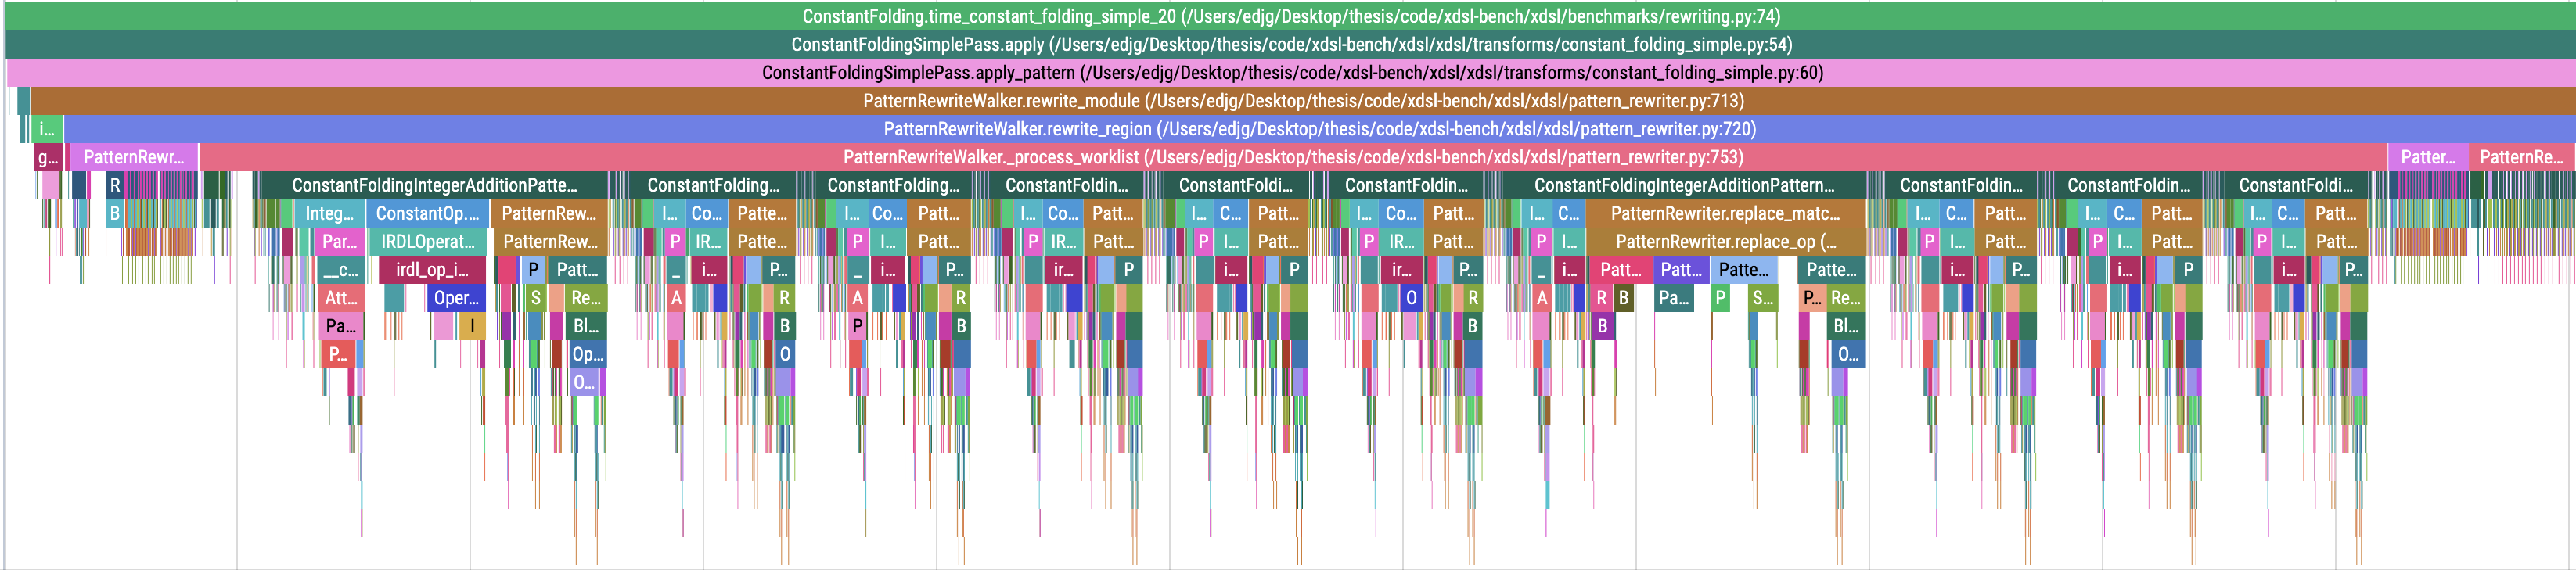
\includegraphics[width=\textwidth]{images/specialising_optimising_xdsl_rewriting/custom_constant_fold.png}
        \captionsetup{width=0.8\textwidth}
        \caption{.}
        \label{fig:constant-fold-original-viztracer}
    \end{subfigure}
    \begin{subfigure}[b]{\textwidth}
        \centering
        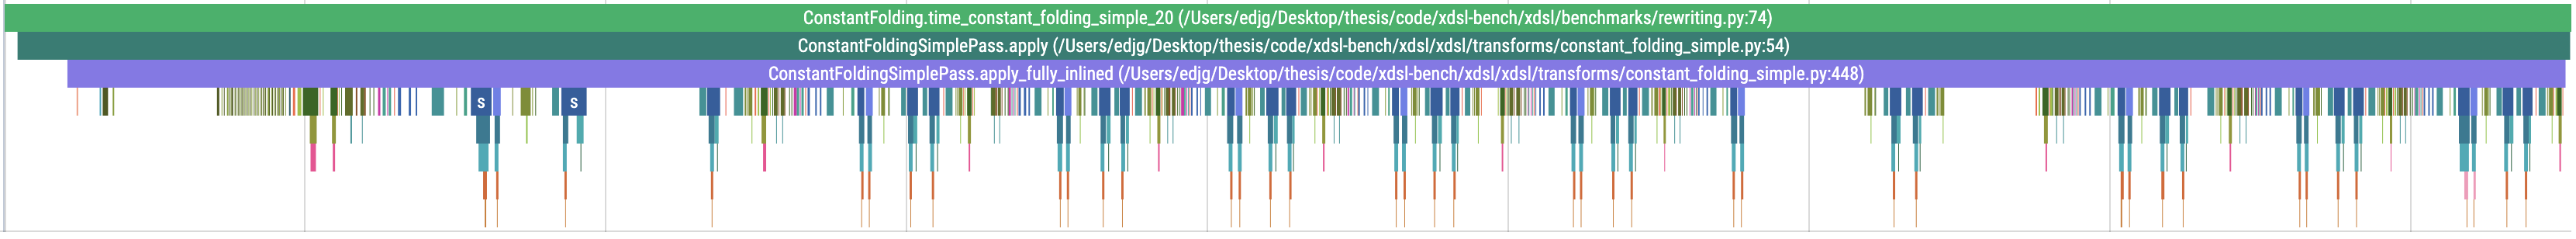
\includegraphics[width=\textwidth]{images/specialising_optimising_xdsl_rewriting/optimised_constant_fold.png}
        \captionsetup{width=0.8\textwidth}
        \caption{.}
        \label{fig:constant-fold-optimised-viztracer}
    \end{subfigure}
    \caption{\texttt{viztracer} traces of.}
    \label{fig:constant-fold-viztracer}
\end{figure}

%% Either perf table here or later in summary?

%% Hopes of automation?
% Link
% Argument
% Link

\subsection{Optimisations}
\label{sec:specialising-pattern-rewriting-optimisations}

%% Introduction + scope of stuff
% Hook
% Argument
% xDSL is very big -- cannot optimise everything! But can show optimisations from specialisation are applicable and make change with time.
% Link


%% Removing overhead in functions
% Link
% Argument
% Link


%% Removing implicit builders
% Link
% Argument
% Link


%% Optional stretch goal to be filled in later...?
%% `__slots__` (stretch dataclasses stuff -> custom dataclass like thing without most of the overhead as a helper, replaces frozen dataclasses (what functionality is used here: https://github.com/python/cpython/blob/main/Lib/dataclasses.py and what can we rip out???))



\subsection{Performance improvement}
\label{sec:specialising-pattern-rewriting-performance}

%% How much did we get out of this?
% Link
% Argument
% Link

%% Figure or table comparing performance
\begin{table}[H]
  \caption{.}
  \label{tab:constant-folding-optimised}
  \centering
  \begin{tabular}{ccc}
    \toprule
    \textbf{MLIR [ns]} & \textbf{xDSL [ns]} & \textbf{Optimised xDSL [ns]} \\
    \midrule
    $3.89 \pm 0.01$ & $504 \pm 76$ & $63.6 \pm 40$\\
    \bottomrule
  \end{tabular}
\end{table}
% Test ConstantFoldingSimple.20(unspecialised) ran in: 0.00115 ± 3e-05s
% Test ConstantFoldingSimple.20(unspecialised) ran in: 0.000142 ± 2.92e-05s
% TODO: This looks wrong...
% SimpleConstantFolding/folding/1           3226 ns         3181 ns       223707
% SimpleConstantFolding/folding/8           5473 ns         5424 ns       131733
% SimpleConstantFolding/folding/64         30174 ns        30110 ns        23037
% SimpleConstantFolding/folding/512       237039 ns       236957 ns         2991
% SimpleConstantFolding/folding/4096     1854095 ns      1853693 ns          379
% SimpleConstantFolding/folding/10000    4584451 ns      4583852 ns          154
% SimpleConstantFolding/folding_BigO      457.63 N        457.56 N
% SimpleConstantFolding/folding_RMS            1 %             1 %


% 7897500000 events in
% mlir::applyPatternsAndFoldGreedily(mlir::Region&, mlir::FrozenRewritePatternSet const&, mlir::GreedyRewriteConfig, bool*)

%% What did we lose from this?
% Link
% Argument
% Link

%% Figure or table comparing lines of code/functionality in some way

%% What does this information let us do?
% Link
% Argument
% Link
